%        File: report.tex
%     Created: Thu Feb 18 01:00 PM 2016 E
% Last Change: Thu Feb 18 01:00 PM 2016 E
%
\documentclass{report}

\usepackage[a4paper, margin=1in]{geometry}

\usepackage{listings}
\usepackage{mathtools}
\usepackage{amsmath}
\usepackage{amssymb}
\usepackage{newlfont}
\usepackage{caption}
\usepackage{subcaption}
\usepackage{titlesec}
\usepackage{empheq}
\usepackage{pdfpages}
\usepackage{enumitem}

\newcommand*\widefbox[1]{\fbox{\hspace{2em}#1\hspace{2em}}}

\newcommand{\eref}[1]{Eq.~(\ref{#1})}
\newcommand{\erefs}[2]{Eq.s~(\ref{#1}-\ref{#2})}
\newcommand{\sk}{\dot{s}_k}
\newcommand{\wk}{\dot{w}_k}
\newcommand{\skg}[1]{{\dot{s}_{#1}}^{(g)}}
\newcommand{\sks}[1]{{\dot{s}_{#1}}^{(s)}}
\newcommand{\kf}[1]{k_{f,#1}}
\newcommand{\kb}[1]{k_{b,#1}}
\newcommand{\kc}[1]{k_{c,#1}}
\newcommand{\kcf}[1]{\frac{k_{f,#1}}{k_{c,#1}}}
\newcommand{\cg}[1]{{C_{#1}^{(g)}}}
\newcommand{\cs}[1]{{C_{#1}^{(s)}}}
\newcommand{\sumk}{\sum_{i=1}^{N_k}}
\newcommand{\ry}{{\rho Y_{k}^{(g)}}}
\newcommand{\yk}{{Y_{k}^{(g)}}}
\newcommand{\dint}[1]{\int_{\Omega}{#1} d \Omega}
\newcommand{\fint}[1]{\int_{\Gamma}{#1} d \Gamma}
\newcommand{\flux}{\vec{F}}
\newcommand{\ma}{\mathbf{A}}

\title{MAE 770 Written Preliminary Exam \#1}

\author{ Kyle B. Thompson }

\begin{document}
\maketitle

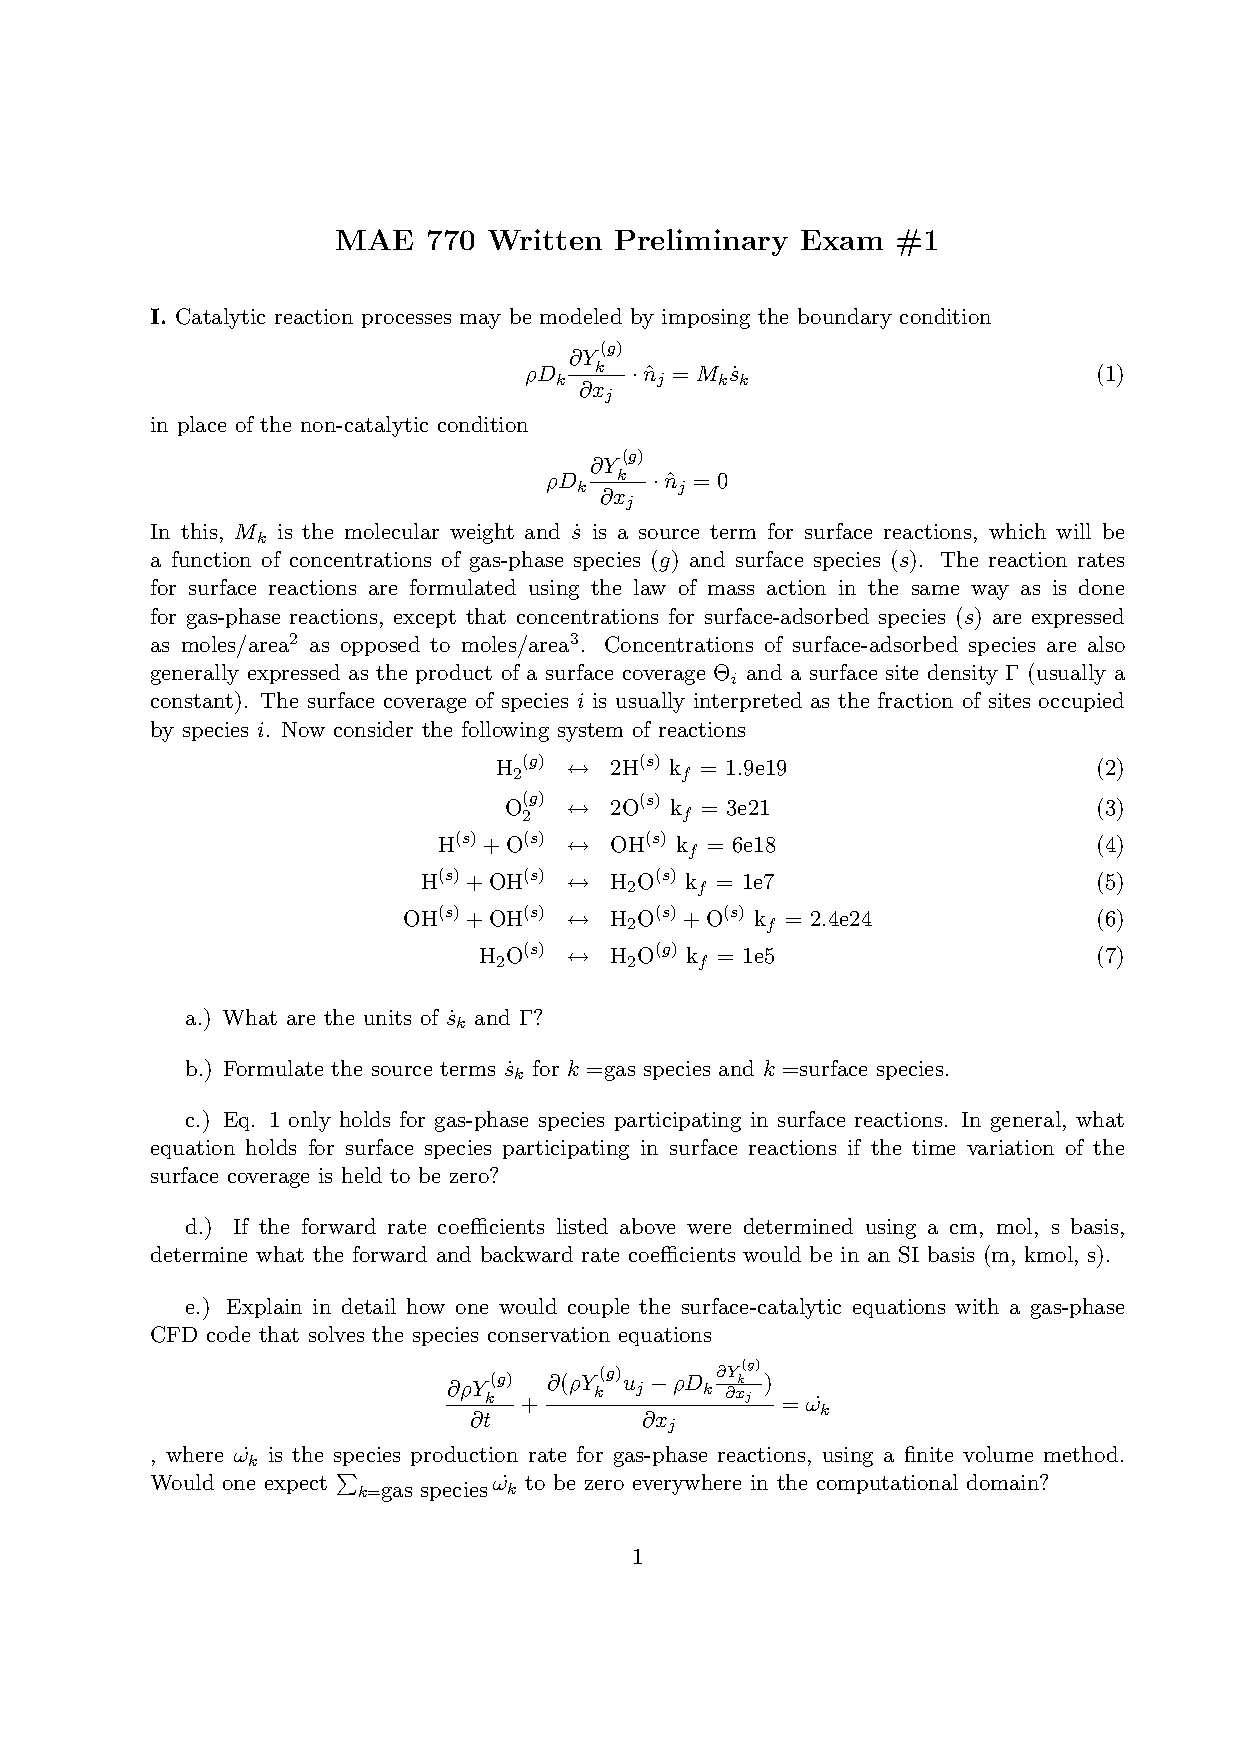
\includepdf{mae770-2016-1.pdf}

\begin{enumerate}[label=(\alph*)]
  \item The units can be determined from the left hand side of the equation
    \begin{equation}
      \rho D_k \frac{\partial Y_k^{(g)}}{\partial x_j} \cdot \hat{n}_j = M_k \sk
      \label{bc-posed}
    \end{equation}
  The units of the variables on the left hand side of \ref{bc-posed} are
  \begin{align*}
    \rho &= \frac{(mass)}{(length)^3} \\
    D_k &= \frac{(length)^2}{(time)} \\
    x_j &= (length)
  \end{align*}
  The mass fraction, $Y_k^{(g)}$, is unitless, as well as the unit normal vector,
  $\hat{n}_j$. Since the units of molecular weight are, $M_k = (mass)/(mole)$, we can
  rearrange \eref{bc-posed} and solve for the units of $\sk$
  \begin{equation}
    \label{units sdot}
    \begin{aligned}
      \sk &= \frac{\rho D_k}{M_k}\frac{\partial Y_k^{(g)}}{\partial x_j}\cdot \hat{n}_j \\
      &= \frac{(mass)}{(length)^3} \frac{(moles)}{(mass)} \frac{(length)^2}{(time)}\frac{1}{(length)} \\
      &= \frac{(moles)}{(length)^2 (time)}
    \end{aligned}
  \end{equation}
  Expressing surface coverage, $\Theta_i$, as the fraction of sites occupied by
  species $i$ implies that it is unitless.  The concentration of
  surface-absorbed species, $C_k$, has units $(moles)/(length)^2$ and must be equivalent to
  the product of surface coverage and surface site density, $\Gamma$; therefore,
  the units of surface site density must be $(moles)/(length)^2$.  Thus, the units for $\sk$
  and $\Gamma$, expressed in the same basis as the problem was posed, are
  \[
    \boxed{\sk = \frac{moles}{area^2-sec}}
  \]
  \[
    \boxed{\Gamma = \frac{moles}{area^2}}
  \]

\item The formulation of the source terms $\sk$ for $k=$ gas species and $k=$
  surface species can be expressed as
  \begin{equation}
    \label{sdot form}
    \begin{gathered}
      \sk = \sum_{r=1}^{N_r}\left[(\nu_{k,r}^{''} - \nu_{k,r}^{'})
      (R_{f,r} - R_{b,r})\right] \\
      R_{f,r} = k_{f,r}\prod_{i=1}^{N_k}(C_i^{\nu_{i,r}^{'}}), \quad
      R_{b,r} = k_{b,r}\prod_{i=1}^{N_k}(C_i^{\nu_{i,r}^{''}})
    \end{gathered}
  \end{equation}
  where $\nu_{k,r}^{'}$ is the stoichometric coefficient for species $k$ in
  reaction $r$ as a reactant in the forward reaction, and $\nu_{k,r}^{''}$ is
  for that species as a product in the forward reaction.  $N_k$ denotes the
  number of species and $N_r$ denotes the number of reactions.  Additionally,
  the backward rate coefficient $k_{b,r}$ is usually determined from the forward
  rate coefficient $k_{f,r}$ and the equilibrium constant $k_{c,r}$.  The later
  of these is often available as a curve fit function of temperature.  Thus,
  using \eref{sdot form} the $\sk$ source terms can be expressed as
  \begin{empheq}[box=\boxed]{align}
    \skg{H_2}  &= -\left( \kf{1} \cg{H_2} - \kcf{1} {\cs{H}}^2 \right) \\
    \skg{O_2}  &= -\left( \kf{2} \cg{O_2} - \kcf{2} {\cs{O}}^2 \right) \\
    \skg{H_2O} &= \left( \kf{6} \cs{H_2O} - \kcf{6} \cg{H_2O} \right) \\
    \begin{split}
      \sks{H}    &= 2 \left( \kf{1} \cg{H_2} - \kcf{1} {\cs{H}}^2 \right) \\
      &-\left( \kf{3} \cs{H} \cs{O} - \kcf{3} \cs{OH} \right) \\
      &-\left( \kf{4} \cs{H} \cs{OH} - \kcf{4} \cs{H_2O} \right)
      \label{H-source}
    \end{split} \\
    \begin{split}
      \sks{O} &= 2 \left( \kf{2} \cg{O_2} - \kcf{2} {\cs{O}}^2 \right) \\
      &-\left( \kf{3} \cs{H} \cs{O} - \kcf{3} \cs{OH} \right) \\
      &+\left( \kf{5} {\cs{OH}}^2 - \kcf{5} \cs{H_2O} \cs{O} \right)
      \label{O-source}
    \end{split} \\
    \begin{split}
      \sks{OH} &= \left( \kf{3} \cs{H} \cs{O} - \kcf{3} \cs{HO} \right) \\
      &-\left( \kf{4} \cs{H} \cs{OH} - \kcf{4} \cs{H_2O} \right) \\
      &-2\left( \kf{5} {\cs{OH}}^2 - \kcf{5} \cs{H_2O} \cs{O} \right)
      \label{OH-source}
    \end{split} \\
    \begin{split}
      \sks{H_2O} &= \left( \kf{4} \cs{H} \cs{OH} - \kcf{4} \cs{H_2O} \right) \\
      &+\left( \kf{5} {\cs{OH}}^2 - \kcf{5} \cs{H_2O} \cs{O} \right) \\
      &-\left( \kf{6} \cs{H_2O} - \kcf{6} \cg{H_2O} \right)
      \label{H2Os-source}
    \end{split}
  \end{empheq}

  \item By characterizing the concentrations of surface species as
    \begin{equation}
      C_i = \theta_i \Gamma
      \label{surface-c}
    \end{equation}
    and differentiating in time
    \begin{equation}
      \frac{\partial C_i}{\partial t} = \frac{\partial \theta_i}{\partial t} \Gamma = \sks{i}
    \end{equation}
    Thus, if the time variation of the surface coverage is held to be zero
    \begin{equation}
      \boxed{
        \begin{aligned}
          \frac{\partial \theta_i}{\partial t} &= \frac{\sks{i}}{\Gamma} = 0 \\
        \end{aligned}
      }
      \label{steady-surf-cov}
    \end{equation}
    For $i$=surface species. This reduces \erefs{H-source}{H2Os-source} to an
    algebraic system to be solved for all surface species concentrations.  The
    algebraic system is nonlinear, and it can be solved by a Newton or
    quasi-Newton iteration in practice.

  \item Determining the units for the forward and backward rate coefficients,
  $k_f$ and $k_b$, begins with looking at the units of $\sk$.  Since the source
  term was found to have units of $moles/(area^2$-$sec)$, in the generic sense, it
  would have proper units of $mol/(cm^2$-$s)$ using a $cm$, $mol$, $s$ basis.
  The units of $k_f$ and $k_b$ will vary for each reaction, but must ultimately
  conform to the fact that $R_{f,r}$ and $R_{b,r}$ in \eref{sdot form} must have
  units of $mol/(cm^2$-$s)$.  For the first reaction
  \begin{equation}
    \kf{1} = 1.9e19 \quad \frac{cm}{s}
    \label{kf_units}
  \end{equation}
  which satisfies
  \begin{equation}
    R_{f,1} = k_{f,1}\cg{H_2} = \frac{cm}{s}\frac{mol}{cm^3} =
    \frac{mol}{cm^2\text{-}s}
    \label{R_units}
  \end{equation}
 More generally, the units for $k_f$ can be expressed as
  \begin{equation}
    \kf{r} = \frac{mol}{(cm^2)(s)\prod_{i=1}^{N_k}\left(
    \left( \frac{mol}{cm^3} \right)^{\nu_{i,r}^{'(g)}} \left( \frac{mol}{cm^2}
    \right)^{\nu_{i,r}^{'(s)}} \right)}
    \label{kf-unit-formula}
  \end{equation}
  where $\nu_{i,r}^{'(g)}$ is the stoichiometric coefficient of gas-phase
  reactant species $i$ in reaction $r$, and $\nu_{i,r}^{'(s)}$ is the
  stoichiometric coefficient of surface reactant species $i$ in reaction $r$.
  Since $R_{b,r}$ must also have units of $mol/(cm$-$s)$, the same reasoning can
  be used to derive
  \begin{equation}
    \kb{r} = \frac{mol}{(cm^2)(s)\prod_{i=1}^{N_k}\left(
    \left( \frac{mol}{cm^3} \right)^{\nu_{i,r}^{''(g)}} \left( \frac{mol}{cm^2}
    \right)^{\nu_{i,r}^{''(s)}} \right)}
    \label{kb-unit-formula}
  \end{equation}
  where $\nu_{i,r}^{''(g)}$ and $\nu_{i,r}^{''(s)}$ are the are the
  stoichiometric coefficients of gas-phase and surface product species $i$ in
  reaction $r$, respectively.  Using \erefs{kf-unit-formula}{kb-unit-formula},
  the units of $\kf{r}$ and $\kb{r}$ (using a $cm$, $mol$, $s$ basis) are
  \begin{align}
    \begin{alignedat}{2}
      \kf{1} &= 1.9e19 && \quad \frac{cm}{s} \\
      \kf{2} &= 3e21   && \quad \frac{cm}{s} \\
      \kf{3} &= 6e18   && \quad \frac{cm^2}{mol\text{-}s} \\
      \kf{4} &= 1e7    && \quad \frac{cm^2}{mol\text{-}s} \\
      \kf{5} &= 2.4e24 && \quad \frac{cm^2}{mol\text{-}s} \\
      \kf{6} &= 1e5    && \quad \frac{1}{s}
    \end{alignedat} \qquad\qquad
    \begin{alignedat}{2}
      \kb{1} &= \kcf{1} \, && \frac{cm^2}{mol\text{-}s} \\
      \kb{2} &= \kcf{2} \, && \frac{cm^2}{mol\text{-}s} \\
      \kb{3} &= \kcf{3} \, && \frac{1}{s} \\
      \kb{4} &= \kcf{4} \, && \frac{1}{s} \\
      \kb{5} &= \kcf{5} \, && \frac{cm^2}{mol\text{-}s} \\
      \kb{6} &= \kcf{6} \, && \frac{cm}{s}
    \end{alignedat}
    \label{kf-kb-cgs}
  \end{align}
  Converting $\kf{r}$ in \eref{kf-kb-cgs} to an SI basis ($m$, $kmol$, $s$),
  using $m = 100\, cm$ and $kmol = 1000\, mol$, yields
  \begin{equation}
    \boxed{\begin{alignedat}{2}
      \kf{1} &= 1.9e17 && \quad \frac{m}{s} \\
      \kf{2} &= 3e19   && \quad \frac{m}{s} \\
      \kf{3} &= 6e17   && \quad \frac{m^2}{kmol\text{-}s} \\
      \kf{4} &= 1e6    && \quad \frac{m^2}{kmol\text{-}s} \\
      \kf{5} &= 2.4e23 && \quad \frac{m^2}{kmol\text{-}s} \\
      \kf{6} &= 1e5    && \quad \frac{1}{s}
    \end{alignedat}}
  \end{equation}
  Using this and \eref{kb-unit-formula}, $\kb{r}$ can also be defined in an SI basis
  \begin{equation}
    \boxed{\begin{alignedat}{2}
      \kb{1} &= \frac{1.9e17 }{\kc{1}}
                \quad && \frac{m^2}{kmol\text{-}s} \\
      \kb{2} &= \frac{3e19   }{\kc{2}}
                \quad && \frac{m^2}{kmol\text{-}s} \\
      \kb{3} &= \frac{6e17   }{\kc{3}}
                \quad && \frac{1}{s} \\
      \kb{4} &= \frac{1e6    }{\kc{4}}
                \quad && \frac{1}{s} \\
      \kb{5} &= \frac{2.4e23 }{\kc{5}}
                \quad && \frac{m^2}{kmol\text{-}s} \\
      \kb{6} &= \frac{1e5    }{\kc{6}}
                \quad && \frac{m}{s}
    \end{alignedat}}
    \label{kb-final}
  \end{equation}
  It should be noted that the equilibrium constants $\kc{r}$ must be in
  an SI basis for the units in \eref{kb-final} to be the correct units of
  $\kb{r}$.  If they in a another basis, then another conversion will be
  necessary.  The conversion of $\kc{r}$ from a $cm$, $mol$, $s$ basis to a $m$,
  $kmol$, $s$ basis can be derived from \erefs{kf-unit-formula}{kb-unit-formula}
  as
  \begin{gather}
    \begin{split}
      \kc{r}^{(cgs)} = \frac{\kf{r}^{(cgs)}}{\kb{r}^{(cgs)}} &= 
      \frac{ \prod_{i=1}^{N_k}\left(
      \left( \frac{mol}{cm^3} \right)^{\nu_{i,r}^{''(g)}} \left( \frac{mol}{cm^2}
      \right)^{\nu_{i,r}^{''(s)}} \right)}
      {\prod_{i=1}^{N_k}\left(
      \left( \frac{mol}{cm^3} \right)^{\nu_{i,r}^{'(g)}} \left( \frac{mol}{cm^2}
      \right)^{\nu_{i,r}^{'(s)}} \right)} \\
      &= \frac{(mol)^a}{ (cm)^b}
    \end{split} \\
    \begin{aligned}
      a &= {\sumk \left(\nu_{i,r}^{''}-\nu_{i,r}^{'} \right)} \\
      b &= {\sumk\left(3{(\nu_{i,r}^{''} - \nu_{i,r}^{'})^{(g)}}
          + 2(\nu_{i,r}^{''} - \nu_{i,r}^{'})^{(s)} \right)} 
    \end{aligned}
  \end{gather}
  \begin{equation}
    \kc{r}^{(mks)} = \kc{r}^{(cgs)}
    \left(\frac{kmol}{1000 \, mol}\right)^a
    \left( \frac{100 \, cm}{m} \right)^b
  \end{equation}
  \item The coupling of the catalytic boundary condition specified in
    \eref{bc-posed} can be accomplished by first examining the finite volume
    (FV) method used.  By integrating and applying the Green-Gauss theorem, the
    species conservation equation can written as
    \begin{equation}
      \frac{\partial}{\partial t}\int_{\Omega}{\ry d \Omega}
      + \fint{\left( \ry u_j - \rho D_k
        \frac{\partial Y_{k}^{(g)}}{\partial x_j}\right) \cdot \hat{n}_j }
      = \dint{\wk}
      \label{continuity}
    \end{equation}
    Where $\Omega$ is a cell volume domain and $\Gamma$ is the
    interface/boundaries of that cell.  For a first order FV scheme, $\ry$ and
    $\wk$ become cell averaged quantities
    \begin{align}
      \overline{\ry} &= \frac{1}{V}\dint{\ry} \\
      \overline{\wk} &= \frac{1}{V}\dint{\wk}
      \label{avg-q}
    \end{align}
    The fluxes at the cell interfaces are discontinuous; therefore, a flux function
    $\flux$ = $\flux (\vec{q}_L, \vec{q}_R)$ is used evaluate fluxes at the cell interface.
    The vectors $\vec{q_{L,R}}$ denote the interface left and right states used
    in evaluating the flux. If \eref{continuity} is integrated explicitly in
    time, $\overline{\ry}$ can be updated via
    \begin{equation}
      (\overline{\ry})_{i}^{n+1} = (\overline{\ry})^{n}_i - \Delta t (R_k)_i
      \label{expl-fv}
    \end{equation}
    Where the superscript $^n$ denotes the time level, the subscript $_i$
    denotes the node or cell number, and $(R_k)_i$ is the residual of species
    $k$ flux at node or cell $i$ computed by summing the fluxes/sources at each
    cell face.  For a node-centered FV method a dual control volume is
    constructed around each node, enabling the residual to be formulated in an
    edge-based fashion.  An advantage of using a node-centered FV method is that
    it is easy to implement the boundary condition posed in \eref{bc-posed} via
    specifying the flux (weak enforcement).  By looping over nodes on the
    boundary with the catalytic surface, the residual can be set by
    \begin{equation}
      (R_k)_{ibc} = \rho D_k \frac{\partial Y_k^{(g)}}{\partial x_j} \cdot \hat{n}_j
      - M_k \sk
      \label{res-bc}
    \end{equation}
    By this weak enforcement of the catalytic boundary condition,
    \eref{bc-posed} is satisfied as the solution of $\overline{\yk}$ converges
    to steady state and $R_k = 0$.

    Since it was previously shown that $\sk$ is a
    function of both the gas phase and surface species concentrations, a
    decision must be made as to how to couple updating the surface-absorbed
    species.  One option is to update the surface species at the same time
    level as the gas phase species have been updated.  While admittedly overly
    simplistic, here is what an implementation of solving one iteration of this
    loosely coupled scheme might look like this

    \begin{lstlisting}[language=FORTRAN, caption=Simple Implementation]

    do timestep = 1, n_timesteps

      ! Form the residual at all nodes
      call add_inviscid_fluxes(q,grid,residual)
      call add_viscous_flux(q,grid,residual)

      ! Set other non-surface boundary conditions
      call set_nonsurface_bc(q,grid,residual)

      ! Set the catalytic boundary condition
      do inode = 1, nsurface_nodes
        bc_node = get_node_on_surface(inode)
        residual(:,bc_node) = set_catalytic_bc(q(:,bc_node), &
                              surface_species(:,bc_node))

      ! Update the surface species concentrations
        sdot = get_surface_source_term(q(:,bc_node))
        surface_species(:,bc_node) = surface_species(:,bc_node) &
                                   + sdot*dt
      end do

      ! Update the conserved (gas-phase) quantities
      do node = 1, nnodes
        q(:,node) = q(:,node) - dt*residual(:,node)
      end do

    end do

    \end{lstlisting}
    In this simple illustration, the gas-phase species mass fractions (or
    densities) are updated to the next time-level, and are in turn used to
    compute the source term vector used to update the surface species
    concentrations via
    \begin{equation}
      \cs{k}^{n+1} = \cs{k}^{n} + \left(\Delta
      t\right)\left(\sk(\cg{k}^{n},\cs{k}^{n})\right)
      \label{cs-update}
    \end{equation}
    for k=surface species.  \eref{cs-update} can also be expressed in terms of
    surface coverage $\cs{k} = \theta_k \Gamma$
    \begin{equation}
      \theta_{k}^{n+1} = \theta_{k}^{n} + \left(\frac{\Delta t}{\Gamma}
      \right)\left(\sk(\cg{k}^{n},\cs{k}^{n})\right)
      \label{theta-update}
    \end{equation}
    As was previously shown, if the time variation of the surface coverage is
    held to be zero, then $\sk = 0$ for k=surface species.  This results in an
    algebraic system of equations to be solved for at the boundary nodes that
    can be solved via a Newton iteration to obtain the surface concentrations.
    In this case, the step of updating and storing the surface species
    concentrations can be handled in the routine ``\verb|set_catalytic_bc|''
    that calculates the boundary flux.  
    
    It is also worth noting that an implicit approach can also be derived
    using a ``loosely coupled'' approach for updating the gas phase and surface
    species. Recasting \eref{continuity} as
    \begin{equation}
      \ma \Delta (\overline{\ry})_i = -(R_k)_i
      \label{implicit-continuity}
    \end{equation}
    Where $\ma$ is the jacobian matrix of the residual fluxes, with the time
    derivative terms on the diagonal.  This becomes a Newton method (or
    quasi-Newton method, depending of the exactness of $\ma$), as the system is
    solved for the state update and marched forward to steady state.  Since
    there is still a need to account for the surface species in this
    formulation, the surface concentrations can be updated with the gas
    concentrations in the overall system; however, this drastically increases
    the number of equations to solve.  This is impractical, since the surface
    concentrations will be zero everywhere other than on the catalytic surface.
    A better approach is to loosely couple the gas-phase system to the surface
    concentrations, where only $\Delta (\overline{\ry})_i$ is solved for at a
    given timestep and the law of mass action can be used to enforce elemental
    conservation in updating the surface concentrations.  In practice, this
    could be done as
    \begin{equation}
      \theta_{k}^{n+1} = \theta_{k}^{n} + \left(\frac{\Delta t}{\Gamma}
      \right)\left(\sk'(\cg{k}^{n+1},\cs{k}^{n})\right)
      \label{theta-update-decoupled}
    \end{equation}
    For $k$ = surface species and $\sk'$ are the source terms from
    \erefs{H-source}{H2Os-source} evaluated such that $\sk$ for $k$ = gas
    species is zero.

    Determining whether the source term components sum to zero is based on
    elemental conservation.  $\sum_{k=\text{gas species}}{\dot{w}_k}$ will only
    be zero everywhere in the computational domain if $\sum_{k=\text{surface
    species}}{\dot{w}_k} = 0$.  If there is production or destruction of surface
    species, then the source terms of the gas-phase species will not sum to
    zero, because this would violate elemental conservation. For example, the
    absorbtion of atomic hydrogen is accounted for in the entire chemical
    species source term, $\sum_{k=\text{all species}}{\dot{w}_k}$, but not in
    just $\sum_{k=\text{gas species}}{\dot{w}_k}$; therefore,
    $\sum_{k=\text{gas species}}{\dot{w}_k} \ne 0$ at the catalytic surface
    boundary. 

\end{enumerate}

\end{document}
